\documentclass[12pt]{article}

\usepackage[utf8]{inputenc}

% Вот эти два пакета для новых шрифтов
\usepackage{mathpazo}
\usepackage{domitian}


\usepackage[T1, T2A]{fontenc}
\usepackage[russian]{babel}
\let\oldstylenums\oldstyle

\usepackage{amssymb,amsmath,mathrsfs,amsthm}

\usepackage{needspace}
\usepackage{wrapfig}
\usepackage{subcaption}
\usepackage{graphicx}
\usepackage[colorlinks,linkcolor=black,citecolor=black, unicode]{hyperref}
\usepackage{indentfirst}

% Параметры страницы
\textheight=24cm
\textwidth=16cm
\oddsidemargin=5mm
\evensidemargin=-5mm
\marginparwidth=36pt
\topmargin=-1cm
\footnotesep=3ex
%\flushbottom
\raggedbottom
\tolerance 3000
% подавить эффект "висячих стpок"
\clubpenalty=10000
\widowpenalty=10000
\renewcommand{\baselinestretch}{1.1}
%\renewcommand{\baselinestretch}{1.5} %для печати с большим интервалом

%math operations
\newcommand{\norm}{\mathop{\rm norm}\limits}
\newcommand{\real}{\mathbb{R}}
\newcommand{\ex}{\mathbb{E}}
\newcommand{\diag}{\mathrm{diag}}
\newcommand{\intset}{\mathrm{int}}
\newcommand{\softmax}{\mathop{\rm softmax}\limits}
\newcommand{\argmin}{\mathop{\rm argmin}\limits}
\newcommand{\lossfunc}{\mathcal{L}'}
\newcommand{\elbo}{\mathcal{L}}
\newcommand{\normal}[3]{\mathcal{N}(#1 | #2, #3)}
\newcommand{\dd}[2]{\frac{\partial#1}{\partial#2}}
\newcommand{\kl}[2]{\mathop{KL}(#1 \parallel #2)}
\newcommand{\nm}{\mathcal{N}}
\newcommand{\sle}{\; \Rightarrow \;}
\newcommand{\indpos}{\mathbf{I}_{d_k}^{+}[i, j]}
\newcommand{\indneg}{\mathbf{I}_{d_k}^{-}[i, j]}


\newcommand{\explanation}{\mathop{\rm explanation}\limits}
%my settings
\graphicspath{{../figures/}}

\begin{document}

\begin{titlepage}
    \begin{center}
        Московский государственный университет имени М. В. Ломоносова
    
        \bigskip
        
\includegraphics[width=50mm]{msu.pdf}
    
        \bigskip
        Факультет Вычислительной Математики и Кибернетики\\
        Кафедра Математических Методов Прогнозирования\\[10mm]
    
        {\large\bfseries
            ДИПЛОМНАЯ РАБОТА СТУДЕНТА 417 ГРУППЫ\\[10mm]
            ''Система визуального анализа для активности головного мозга''}
        \\[80mm]
        
    
        \begin{flushright}
            \parbox{0.4\textwidth}{
                Выполнил:\\
                студент 4 курса 417 группы\\
                \emph{Тыцкий Владислав Игоревич}\\[5mm]
                Научный руководитель:\\
                к.ф-м.н., доцент\\
                \emph{Майсурадзе Арчил Ивериевич}
            }
        \end{flushright}
    
        \vspace{\fill}
        Москва, 2021
    \end{center}
\end{titlepage}


\section*{Аннотация}
--В последнюю очередь--

\newpage

\tableofcontents

\newpage

\section{Введение}
-- В последнюю очередь --

\section{Методы интерпретации моделей машинного обучения}
Методы интерпретации моделей машинного обучения можно поделить на:

\begin{itemize}
    \item Восприятие объекта:
        \begin{itemize}
            \item Локальные -- объясняют поведение модели для конкретного объекта. 
            \item Глобальные -- объясняют работу модели в целом на всей выборке.
        \end{itemize}

    \item Восприятие модели:
        \begin{itemize}
            \item Агностичные к модели (Model Agnostic) -- алгоритм интерпретации не опирается на
            внутреннюю структура модели. 
            Все, что видит агностичная модель -- это пару ''вопрос'' ''ответ'' или 
            в терминах машинного обучения $(x_i,y_i)$.
            \item  Специфичные для модели (Model Specific) -- учитывая специфику изучаемой модели, 
            мы можем придумать алгоритм, работающий лучше(качественней, быстрее)
            чем агностичные методы интерпретации.
        \end{itemize}
\end{itemize}
\subsection{Специфичные для модели (Model Specific)}
Как упоминалось выше, методы интерпретации специфичные для модели опираются на ее внутреннюю структуру.
Одним из простейших методов интерпретации для линейной модели может послужить рассмотрение весов для каждого признака -- 
мы считаем, что чем больше(по модулю) вес у признака, тем более важным он является для предсказания. Более того, если вес,
соответствующий признаку имеет положительное/отрицательное значение, можно говорить о положительной/отрицательной ''корреляции'' между этим признаком $x_i$ и
целевым значением $y_i$. 

$$ 
y_i = f(<x_i, w>) \text{\textit{, где}}~ f(x) = x ~\text{\textit{или}}~ f(x) = sign(x)
$$

Важно отметить, что все признаки должны иметь одинаковое матожидание и дисперсию. 
Иначе веса для каждого признака могут зависеть от абсолютных значений признака, а не от его важности для модели.
Можно сказать, что линейная модель интерпретируема сама по себе, мы считаем, что принцип ее работы настолько прост, что 
сама внутренняя структура модели (веса признаков) может объяснить ее поведение. 

\newpage
\noindent
Достоинства линейных моделей:
\begin{itemize}
    \item Вес модели в значительной мере определяет важность признака и этим можно пользоваться в качестве интерпретации
    \item Хорошо изучены и ''понимаемы'' сообществом 
    \item Использование как ''суррогатной'' модели \footnote{Далее мы приведем пример суррогатной модели (LIME)}
\end{itemize}

\noindent
Недостатки линейных моделей:
\begin{itemize}
    \item Обобщающей способности далеко не всегда достаточно для получения модели с надлежащим качеством
    \item Зависимость весов от других факторов (например от абсолютных значений признака)
\end{itemize}

\begin{figure}[htb]
    \centering
    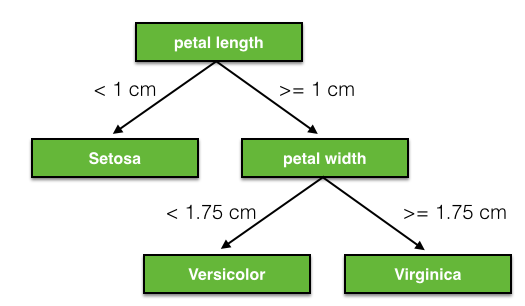
\includegraphics[width=0.5\linewidth]{decision_tree_0.png}
    \caption{Принцип работы решающего дерева}
    \label{decision_tree}
\end{figure}

Еще одним примером интерпретации специфичной для модели может послужить интерпретация решающего дерева. 
Решающее правило f, по которому для $x_i$ сопоставляется $y_i$ весьма близко к тому, как рассуждает человек, когда принимает какие-либо решения.
На каждом этапе мы рассматриваем конкретный признак и исходя из значения этого признака для объекта ''спускаемся'' в соответствующий узел. 

\noindent
Конкретный метод построения решающего дерева обычно определяется:\footnote{Мы не будем подробно останавливаться на особенностях построения деревьев решений}
\begin{itemize}
    \item Видом предикатов в вершинах.
    \item Критерием информативности Q.
    \item Критерием останова.
\end{itemize}

\newpage
\noindent
Достоинства деревьев решений:
\begin{itemize}
    \item Разделяет данные на отдельные группы, что проще воспринимать, 
    чем гиперплоскости больших размерностей 
    \item Естественная визуализация метода
    \item Решающее правило сходно с тем, как рассуждает человек
\end{itemize}

\noindent
Недостатки деревьев решений:
\begin{itemize}
    \item Плохо справляются с линейными зависимостями
    \item Легко переобучаются(дерево, где в каждом листе один объект)
    \item Чем больше дерево, тем сложнее его интерпретировать 
\end{itemize}




\subsection{Агностичные модели (Model Agnostic)}
Большим преимуществом методов интерпретации, не зависящих от модели,
по сравнению с методами интерпретации, специфичными для конкретной модели, 
является их гибкость. Методы интерпретации могут быть 
применены к любой модели, поэтому исследователи могут свободно использовать 
любую модель, которая им нравится. Все, что основывается на интерпретации модели машинного обучения, 
например графический или пользовательский интерфейс, также становится независимым от базовой 
модели машинного обучения. Как правило, для решения задачи оценивается не один, а множество типов
моделей машинного обучения, и при сравнении моделей с точки зрения интерпретируемости легче работать
с объяснениями, не зависящими от модели, поскольку один и тот же метод может быть использован для любого
типа модели.

\vspace{10pt}
\noindent
Желаемые свойства агностического метода интерпретации:
\begin{itemize}
    \item Гибкость модели -- метод интерпретации может работать с любой моделью машинного обучения,
    такой как бустинги, случайные леса,и нейронные сети.
    \item Гибкость объяснения -- мы не ограничены определенной формой объяснения. В некоторых случаях может 
быть полезно взглянуть на важности всех признаков, а в других выделить область изображения на картинке,
являющийся причиной именно такого ответа.
    \item Гибкость представления -- система должна иметь возможность работать с различным
    представлением объектов, будь то текст, картинка или табличные данные.
\end{itemize}

\subsection{LIME}
Локальные суррогатные модели(Local surrogate models) -- это модели, которые можно использовать
для объяснения отдельных прогнозов других моделей \textit{''черных ящиков''.}\footnote{Термин
''черный ящик'' можно воспринимать как модель, о структуре которой мы ничего не знаем. Все, что 
мы можем: 1) Подать на вход модели объект из обучающей выборки, 2) Получить предсказание модели}

В статье "Why I should trust you?"\cite{Lime} -- авторы предлагают конкретную реализацию локальных суррогатных моделей.
Суррогатные модели обучаются для аппроксимации прогнозов ''черного
ящика''. Цель локальных суррогатных моделей -- понять, почему ''черный ящик'' сделал определенный прогноз на конкретном объекте. 
LIME изучает, что происходит с прогнозами, когда мы некоторым образом меняем объекты из обучающей выборки.
LIME генерирует новый набор данных, состоящий из ''возмущенных'' выборок и соответствующих им прогнозов.
На этом новом наборе данных обучается интерпретируемая модель, 
которая взвешивает объекты пропорционально близости к объекту, для которого мы объяснить поведение модели. 
Интерпретируемой моделью может быть что угодно, например линейная модель или дерево решений. 

\vspace{10pt}
\noindent
Математически локальные суррогатные модели выражаются следующим образом:

$$\explanation(x) = \argmin\limits_{g \in G}L(f, g, \pi_x) + \Omega(g)$$

$$L(f,g,\pi_x) = \sum\limits_{x'} (f(x') - g(x'))^2\pi_x(x,x')$$

\noindent
где $g$ (например, линейная модель), минимизируюшая функцию потерь $L$ (например MSE), которая 
измеряет, насколько близки прогнозы $g$ к прогнозу исходной модели - ''черному ящику'' f, 
а $|Omega(g)$  -- это сложность модели. G - это семейство возможных
интерпретируемых моделей, например, всевозможные линейные модели. Мера близости  
$\pi(x)$ определяет окрестность вокруг объекта x, которую мы рассматриваем для построения объяснения. 

\begin{figure}[htb]
    \centering
    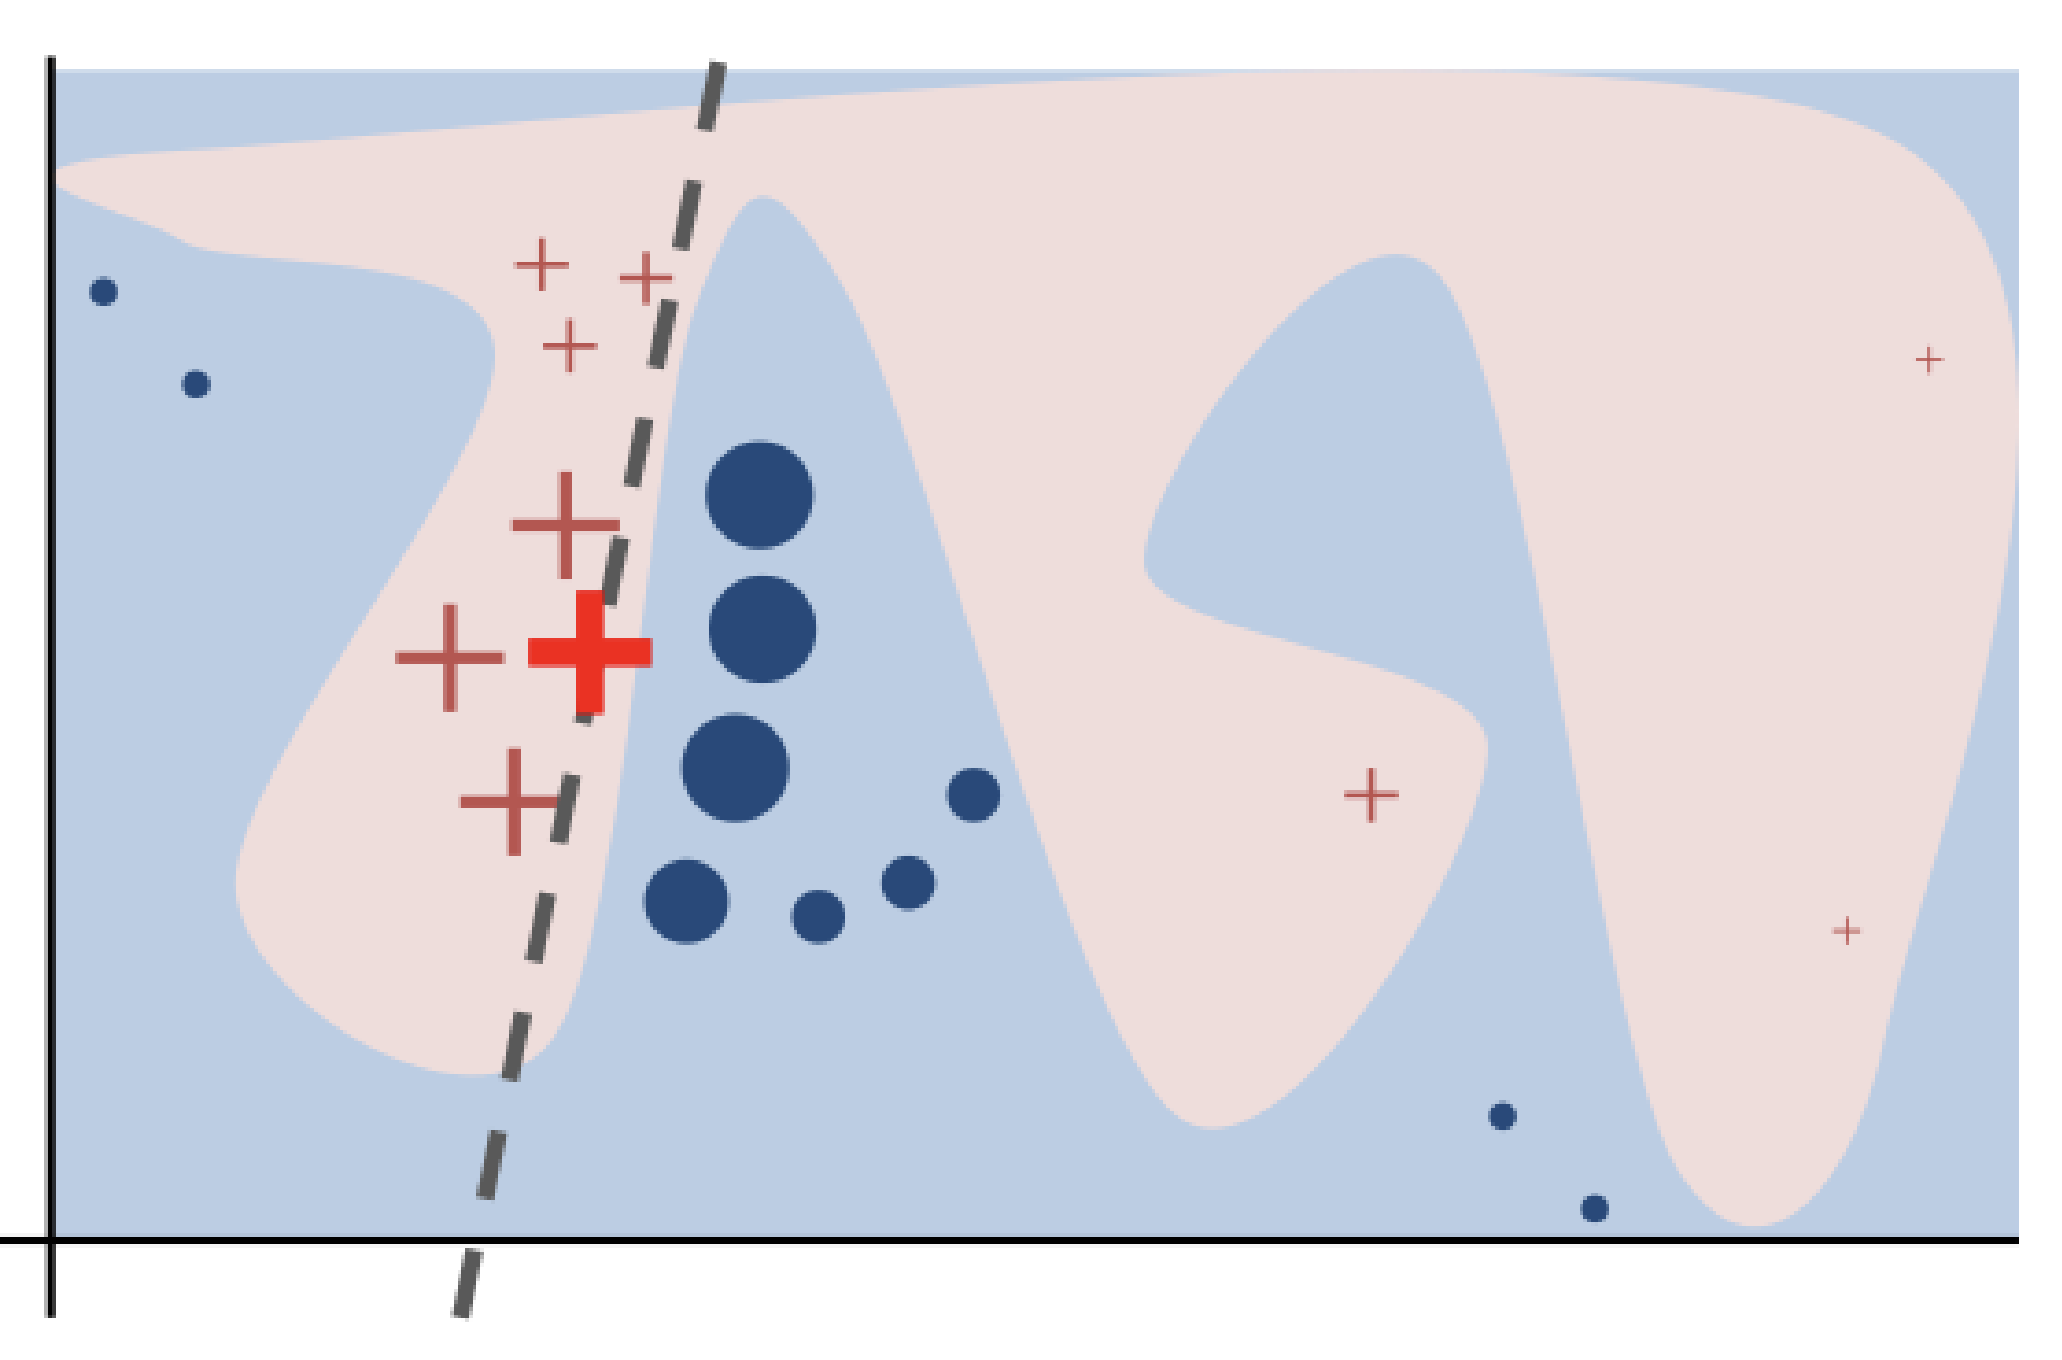
\includegraphics[width=0.8\linewidth]{lime_from_article.png}
    \caption{Принцип работы LIME}
    \label{lime_from_article}
\end{figure}


Шаги для обучения локальных суррогатных моделей:

\begin{enumerate}
    \item Выбрать интересующий вас объект, 
    для которого нужно получить объяснение предсказания от модели - ''черного ящика''.
    \item Получить предсказания на других объекта выборки (выборку можно создать искусственно).
    \item Взвесить объекты в соответствии с их близостью к интересующему объекту.
    \item Обучить взвешенную, интерпретируемую модель на этом наборе данных.
    \item Объяснить прогноз, интерпретируя локальную модель.
\end{enumerate}

Как вы можно получить ''возмущенные'' данные? Это зависит от типа объектов, которые
могут быть текстовыми, графическими или табличными. 
Для текста и изображений решение состоит в том, чтобы включать или 
выключать отдельные слова или ''суперпиксели''. В случае табличных данных 
LIME создает новые выборки с помощью небольших изменений уже существующих объектов. К примеру,
если все признаки объекта являются числовыми, то можно сгенерировать новые данных в некоторой окрестности объектов.

\subsection{SHAP}
-- Понятно, что писать --
\subsection{DEEP Lift/Gradient based методы}
-- Слышал, но пока что не изучал --

\section{Существующие методы интерпретации временных рядов}
Название не вполне удачное -- часто интерпретацией временных рядов называют
разложение его на компоненты: сезонность, тренд и т.д.

\section{Предлагаемые методы}
Задачи seq2seq, seq2label, быть может другие задачи 
\subsection{''Суперпризнаки''}
-- +- Понятно, что писать, но нужно проводить эксперименты --
\subsection{CNN}
-- +- Понятно, что писать, но нужно проводить эксперименты --
\subsection{Графовые нейросети}
--  Пока непонятно, что писать, нужно проводить эксперименты --

\section{Применение к временным рядам}
\subsection{Активность головного мозга}
-- С данными туговато пока что --

Да и в принципе пока что не получается красной нитью вплести
эту тему в текст
\subsection{Другие примеры}
-- Здесь много разного можно напридумывать --

\section{Заключение}
--В последнюю очередь--

\section{Полезные ссылки}

\begin{itemize}
    \item \url{https://arxiv.org/pdf/1909.07082.pdf}  хорошая статья, приведен метод оценивания качества XAI
    \item \url{https://arxiv.org/pdf/2009.13211.pdf} Хорошая статья, предложен соверешенно другой метод объяснения временных рядов
    \item \url{https://proceedings.neurips.cc/paper/2020/file/2c29d89cc56cdb191c60db2f0bae796b-Paper.pdf} просто обзор методов для разных областей 

    \item \url{https://boa.unimib.it/retrieve/handle/10281/324847/492202/Manuscript.pdf} возможно что-то полезное, не читал пока что
    \item \url{https://arxiv.org/pdf/2109.12935.pdf} обзор методов для временных рядов
\end{itemize}

\url{https://github.com/marcoancona/DeepExplain}
\url{https://mne.tools/stable/auto_tutorials/preprocessing/40_artifact_correction_ica.html} -- красивые картинки с головами

\subsection{Датасеты}
 ECG hearbeat dataset -- sec2label
 
 UCR Time Series Classification Archive -- очень много разного
 
 \url{https://github.com/lmmentel/awesome-time-series} -- очень много разного
 
 \url{https://github.com/bhimmetoglu/time-series-medicine} -- три датасета
 
 Human Activity Recognition  -- sec2label
 
 Physionet MIT BIH Arrhythmia -- ???
 
 \url{https://github.com/bhimmetoglu/time-series-medicine/tree/master/EEG} -- sec2label(EEG)
 
 EEG Eye State DataSet -- sec2label
 
\url{https://github.com/effervescent-shot/Dream-Prediction} -- sec2sec (EEG)


\begin{thebibliography}{9}
    \bibitem{Lime}
    Ribeiro M. T., Singh S., Guestrin C. " Why should i trust you?" 
    Explaining the predictions of any classifier //Proceedings of the 22nd ACM SIGKDD 
    international conference on knowledge discovery and data mining. – 2016. – С. 1135-1144.

    \bibitem{scrabble_gan}
    Fogel S. et al. Scrabblegan: Semi-supervised varying length handwritten
    text generation //Proceedings of the IEEE/CVF Conference on 
    Computer Vision and Pattern Recognition. – 2020. – С. 4324-4333.

    \bibitem{dan}
    Wang T. et al. Decoupled attention network for text recognition 
    //Proceedings of the AAAI Conference on Artificial Intelligence. – 2020. – Т. 34. – №. 07. – С. 12216-12224.

    \bibitem{chd}
    www.kaggle.com/constantinwerner/cyrillic-handwriting-dataset

    \bibitem{hkr}
    github.com/abdoelsayed2016/HKR\_Dataset

    \bibitem{iam}
    https://fki.tic.heia-fr.ch/databases/iam-handwriting-database

\end{thebibliography}

\end{document}